%\documentclass[journal]{vgtc}                % final (journal style)
%\documentclass[review,journal]{vgtc}         % review (journal style)
%\documentclass[widereview]{vgtc}             % wide-spaced review
\documentclass[preprint,journal]{vgtc}       % preprint (journal style)

%% Uncomment one of the lines above depending on where your paper is
%% in the conference process. ``review'' and ``widereview'' are for review
%% submission, ``preprint'' is for pre-publication, and the final version
%% doesn't use a specific qualifier.

%% Please use one of the ``review'' options in combination with the
%% assigned online id (see below) ONLY if your paper uses a double blind
%% review process. Some conferences, like IEEE Vis and InfoVis, have NOT
%% in the past.

%% Please note that the use of figures other than the optional teaser is not permitted on the first page
%% of the journal version.  Figures should begin on the second page and be
%% in CMYK or Grey scale format, otherwise, colour shifting may occur
%% during the printing process.  Papers submitted with figures other than the optional teaser on the
%% first page will be refused. Also, the teaser figure should only have the
%% width of the abstract as the template enforces it.

%% These few lines make a distinction between latex and pdflatex calls and they
%% bring in essential packages for graphics and font handling.
%% Note that due to the \DeclareGraphicsExtensions{} call it is no longer necessary
%% to provide the the path and extension of a graphics file:
%% 
\includegraphics{diamondrule} is completely sufficient.
%%
\ifpdf%                                % if we use pdflatex
  \pdfoutput=1\relax                   % create PDFs from pdfLaTeX
  \pdfcompresslevel=9                  % PDF Compression
  \pdfoptionpdfminorversion=7          % create PDF 1.7
  \ExecuteOptions{pdftex}
  \usepackage{graphicx}                % allow us to embed graphics files
  \DeclareGraphicsExtensions{.pdf,.png,.jpg,.jpeg} % for pdflatex we expect .pdf, .png, or .jpg files
\else%                                 % else we use pure latex
  \ExecuteOptions{dvips}
  \usepackage{graphicx}                % allow us to embed graphics files
  \DeclareGraphicsExtensions{.eps}     % for pure latex we expect eps files
\fi%

%% it is recomended to use ``\autoref{sec:bla}'' instead of ``Fig.~\ref{sec:bla}''
\graphicspath{{figures/}{pictures/}{images/}{./}} % where to search for the images

\usepackage{float}
\usepackage{microtype}                 % use micro-typography (slightly more compact, better to read)
\PassOptionsToPackage{warn}{textcomp}  % to address font issues with \textrightarrow
\usepackage{textcomp}                  % use better special symbols
\usepackage{mathptmx}                  % use matching math font
\usepackage{times}                     % we use Times as the main font
\renewcommand*\ttdefault{txtt}         % a nicer typewriter font
\usepackage{cite}                      % needed to automatically sort the references
\usepackage{tabu}                      % only used for the table example
\usepackage{booktabs}                 % only used for the table example

%% We encourage the use of mathptmx for consistent usage of times font
%% throughout the proceedings. However, if you encounter conflicts
%% with other math-related packages, you may want to disable it.

%\inputencoding{latin1}
%% In preprint mode you may define your own headline.
%\preprinttext{To appear in IEEE Transactions on Visualization and Computer Graphics.}

%% If you are submitting a paper to a conference for review with a double
%% blind reviewing process, please replace the value ``0'' below with your
%% OnlineID. Otherwise, you may safely leave it at ``0''.
\onlineid{0}

%% declare the category of your paper, only shown in review mode
\vgtccategory{Research}
%% please declare the paper type of your paper to help reviewers, only shown in review mode
%% choices:
%% * algorithm/technique
%% * application/design study
%% * evaluation
%% * system
%% * theory/model
\vgtcpapertype{application/design study}

%% Paper title.
\title{Exploring potential causes, consequences and visualizing evolution of major air pollutant emissions over EU28}

%% This is how authors are specified in the journal style

%% Les auteurs 
\author{Jules Sauvinet, Marine Ruiz}
\authorfooter{
%% insert punctuation at end of each item
\item
 Jules Sauvinet is studying at Universit\'e Claude Bernard Lyon I. E-mail: contact@julessauvinet.fr.
\item
 Marine Ruiz is studying at Universit\'e Claude Bernard Lyon I. E-mail: marine.ruiz@etu.univ-lyon1.fr.
}

%other entries to be set up for journal
%\shortauthortitle{Biv \MakeLowercase{\textit{et al.}}: Global Illumination for Fun and Profit}
%\shortauthortitle{Firstauthor \MakeLowercase{\textit{et al.}}: Paper Title}

%% Abstract section.
\abstract{
From now on, the media talks about environmental issues on a daily basis. Pollution peaks have become commonplace in large metropolises and air pollution is becoming a subject that is increasingly affecting citizens. As pollution is not only a visual or olfactory discomfort, it is now the main environmental health risk in the world. On average, it causes the premature death of 7 million people worldwide, including 600 000 in Europe and more than 50 000 in France, according to the World Health Organization, the Ministry of the Environment and the Environment. European Environment Agency.
We propose here a model which allows to visualize the evolution of the emissions of the main harmful pollutants during 12 years and to explore the potential causes and consequences. For instance, does it seems to be an obvious correlation between the fines particles emissions and pulmonary diseases?
}

%% Keywords that describe your work. Will show as 'Index Terms' in journal
%% please capitalize first letter and insert punctuation after last keyword
\keywords{Air pollution, Pollutant, Ammoniac, Sulphur oxides, Non-methane volatil organic compounds, Nitrogen oxides, Particule matters, EU28, Ecology, Health.}

%% ACM Computing Classification System (CCS). 
%% See <http://www.acm.org/class/1998/> for details.
%% The ``\CCScat'' command takes four arguments.
\CCScatlist{ % not used in journal version
 \CCScat{Human-centered computing}{Visualization}%
{Visualization application domains}{Geographic visualization};
}


%% Uncomment below to include a teaser figure.
\teaser{
  \centering
  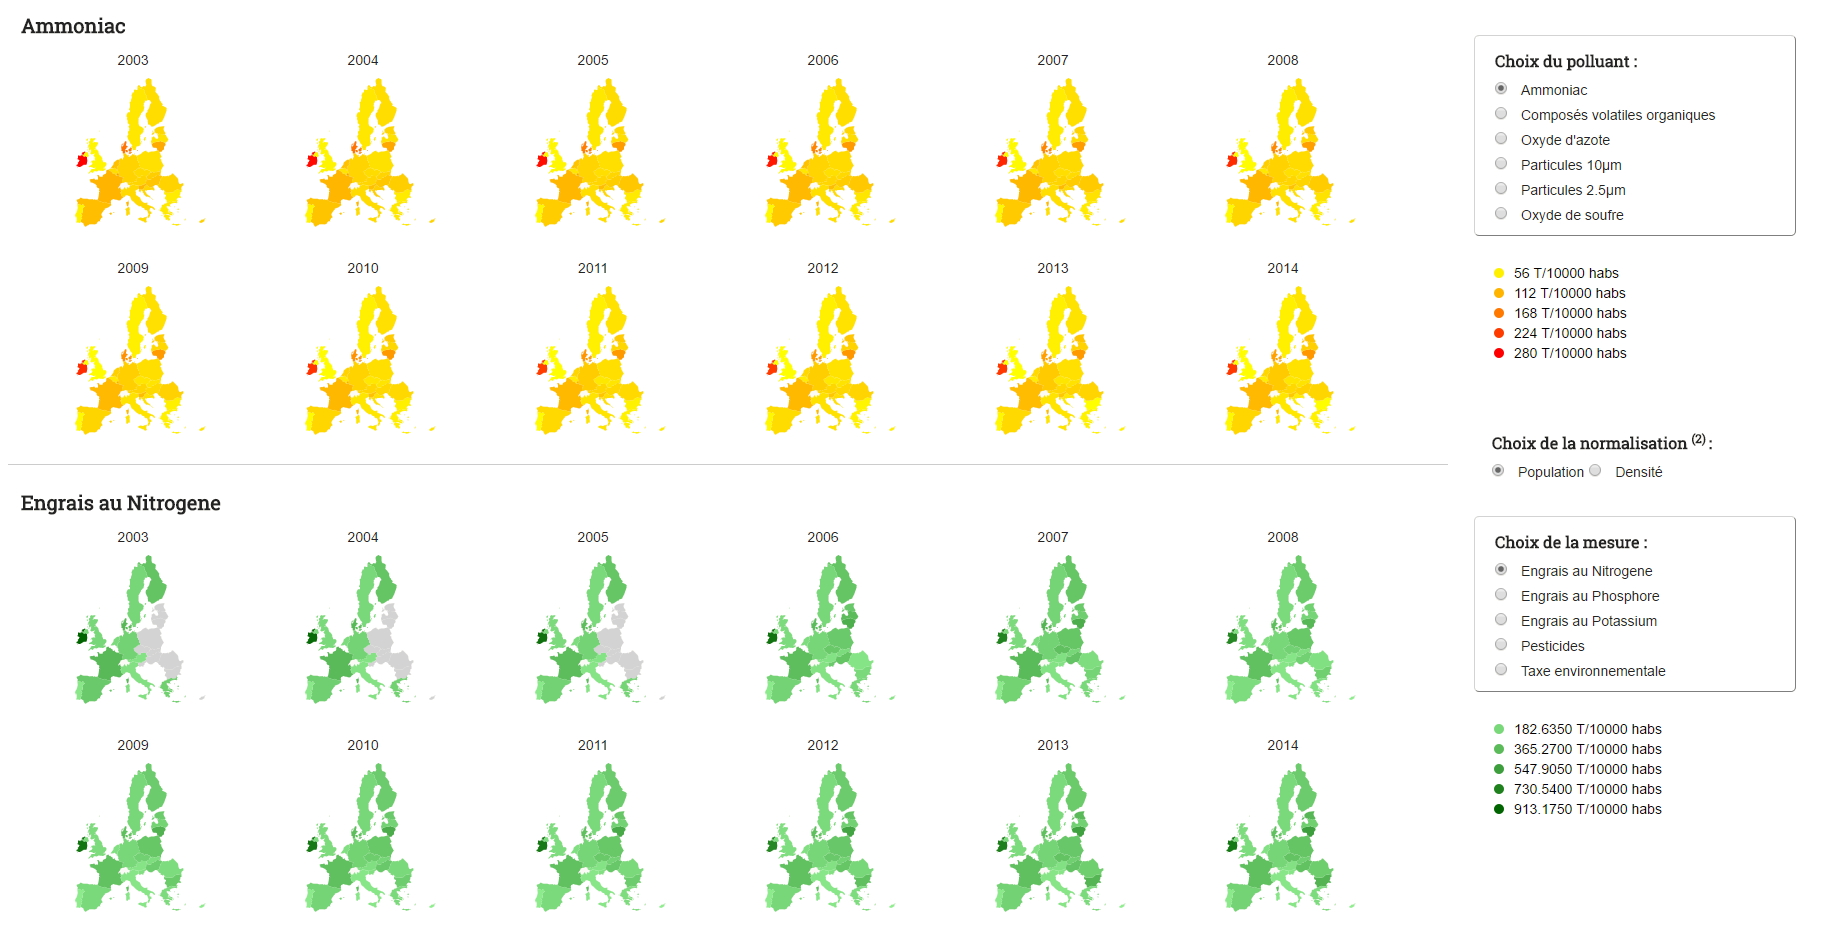
\includegraphics[width=\linewidth]{teaserView}
  \caption{Main view of the visualization: 12 small maps of EU28 colored according to ammoniac emissions on the top and 12 small maps of EU28 showing quantity used of Nitrogen fertilizers from 2003 to 2014.}
	\label{fig:teaser}
}

%% Uncomment below to disable the manuscript note
%\renewcommand{\manuscriptnotetxt}{}

%% Copyright space is enabled by default as required by guidelines.
%% It is disabled by the 'review' option or via the following command:
% \nocopyrightspace

\vgtcinsertpkg

%%%%%%%%%%%%%%%%%%%%%%%%%%%%%%%%%%%%%%%%%%%%%%%%%%%%%%%%%%%%%%%%
%%%%%%%%%%%%%%%%%%%%%% START OF THE PAPER %%%%%%%%%%%%%%%%%%%%%%
%%%%%%%%%%%%%%%%%%%%%%%%%%%%%%%%%%%%%%%%%%%%%%%%%%%%%%%%%%%%%%%%

\begin{document}

%% The ``\maketitle'' command must be the first command after the
%% ``\begin{document}'' command. It prepares and prints the title block.

%% the only exception to this rule is the \firstsection command
\firstsection{Introduction}

\maketitle

\paragraph{}
The emissions of most harmful air pollutants has globally decreased over the past 25 years in European Union (see the \autoref{fig:pollution_decrease} below).
Nevertheless, emissions remain very high, particularly in some countries whose economy depends on sectors responsible for the discharge of certain pollutants. While some countries have taken stock of the issue and taken steps to reduce their emissions, others are struggling to keep pace with economic and political conflicts.
As a result, there are regularly many pollution peaks in major European cities, posing serious problems for the environment and health.

\begin{figure}[H]
 \centering % avoid the use of \begin{center}...\end{center} and use \centering instead (more compact)
 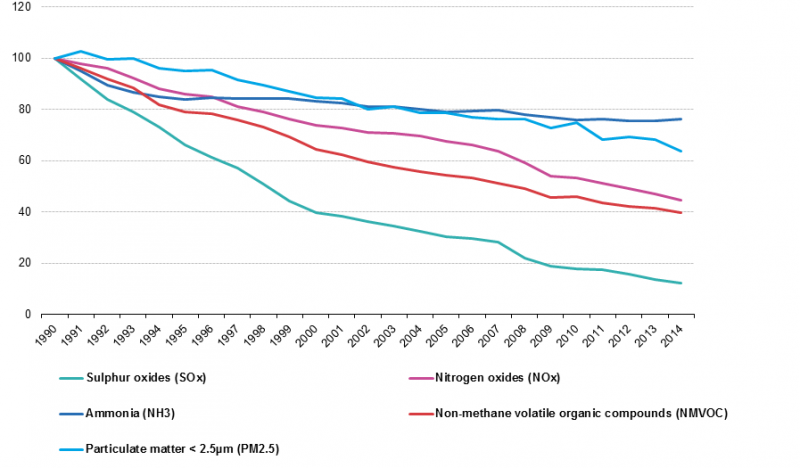
\includegraphics[width=\columnwidth]{decreased_emissions}
 \caption{A visualization of pollution over EU28 for the past 25 years. The image is from \cite{Eurostats:2016:VMC} and is in the public domain.}
 \label{fig:pollution_decrease}
\end{figure}

\paragraph{}
The model we are proposing has two parts.

\paragraph{}
The first part is to be able to visualize the evolution of pollution in the European Union countries for 6 pollutants identified by Eurostats as among the most dangerous for the environment and health: Ammonia (NH3), Sulfur Oxides (SOx) Nitrogen Oxides (NOx), Non-methane volatile organic compounds (NMVOC), Fine Particles less than 2.5um (PM2.5), and Fines Particles less than 10um (PM10).

\paragraph{}
In order to be able to visualize the evolution of the emission of these pollutants, we have developed an interface composed of 12 small maps from the European Union countries to 28 concerning 12 recent years (the data we have of the pollutants range from 1990 to 2014, and these are more complete the longer the time). The user chooses the pollutant from which he wishes to consult changes in the list of 6 specified earlier. Then, each small map (see the \autoref{fig:smallmapammoniac} below) is colored according to a scale of color more or less intensely depending on the amount of pollution rejected per inhabitant. The countries whose data we do not have are colored gray. The color scale is constructed from two minimum and maximum values ​​which are the minimum and maximum rejected pollution values ​​by a country during the 12 years considered.

\paragraph{}
Thus, the user can observe the evolution of the pollution to compare the countries between two countries or for the same country for two different years. The small maps give him an overview showing the general trend of the evolution of pollution for the 12 years and the pollutant considered. Moreover, the color scale makes it possible to isolate clearly the countries which have a much higher emission than the others (e.g. Ireland in figure 3).

\begin{figure}[H]
 \centering % avoid the use of \begin{center}...\end{center} and use \centering instead (more compact)
 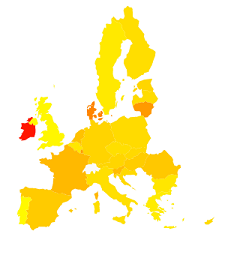
\includegraphics[width=130px]{smallmap}
 \caption{A visualization of a small map. The image is from our visualisation.}
 \label{fig:smallmapammoniac}
\end{figure}

\paragraph{}
The second part of our model is the exploration of the potential causes and consequences of pollution among those that we propose. Once the pollutant has been chosen, the user can choose from a list what we will call a comparison measure. For example, for ammonia, the user can choose from the "Nitrogen Fertilizer" measure. A second set of 12 small maps is then made showing this time the evolution of the measure considered for the maximum 12 years common with those of the pollutants whose data are available.

\paragraph{}
Thus, by comparing the intensity of the coloration of the two series of small maps, the user can identify if there is a potential link between the pollutant and the measure considered. First, it is possible to observe if over a year the color nuances correspond and potentially indicates a correlation for the target year. Secondly, it is possible to observe whether the evolution trends (growth, decay, stagnation) are connected (similar, or opposite). The goal is to invite the user to wonder but obviously does not affirm the observed link.

\newpage
%% \section{Introduction} %for journal use above \firstsection{..} instead


\section{Related Work}

\begin{itemize}
\item In his visualisation \cite{Boy:2014:TCP}, Boy and Fekete shows C02 emissions in countries around the world as clouds of visual smoke. The visualization is reused here \cite{Mediapart:2014:CPM} as a narrative visualization. The literature in InfoVis (Information Visualization) often states that a narrative visualization (storytelling) can engage the reader in data mining. The visualization allows an exploration in time and the comparison of emission between the different countries. But the reader must take the time to "read the visualization". In addition, it is not possible to directly compare the issue between two years.
%http://peopleviz.gforge.inria.fr/trunk/data_blog/environment/co2_FR/index_storytelling.php

\item The concept of displaying a serie of small maps is also known as small multiples as popularized by Tufte \cite{Tufte:1983:VDQ}. In his article \cite{Smith:2005:MSM}, Smith show the interest of small multiples maps for geographical and time visualization. He says that multiple small maps may prove useful as a method of data visualization and/or seeking. Furthermore, according to him, small multiples maps have the potential to address the problem of highly dimensional data, and simplify searches for information over time.

\item In this article \cite{Reimer:2011:SSM}, the authors show how small multiples maps might be useful to complete the task in of comparison of the variation of data values over other variables. They say that small multiples of a geographical map is relevant to obtain to compare different spatial configurations of values.

\item In his article \cite{Few:2009:GDV}, Stephen Few talks about choropleth maps and the use of color intensity for displaying quantities.

\item In this article \cite{Eurostats:2016:VMC}, from the website "http://ec.europa.eu/" where we pick our data, a study of the evolution of the pollutants of our visualization is presented with an explanation of the emitting sectors. The format of this kind of article does not have the catchy side that we want to have with our visualization.

\item Here \cite{Brewer:1994:CUG} , Brewer talks about the adapted colors to use for mapping and visualization.


\end{itemize}

\newpage



\section{Project Description (2p)}
\paragraph{}
	\subsection{Web Page description}
	\paragraph{}
We organized our Web Page into 3 parts:  first, a header which describes the project, then an area with 12 small maps of the European countries, showing pollution-related data, thanks to the pollutant list, the legend and the colors. On the top of this area, there is a title which displays the name of the pollutant. Finally, an other area with the same 12 small maps, this time to show pollutant-related data such as causes, consequences or correlations to the emission of the pollutant selected.
\paragraph{}
To be more accurate, next to the 12 pollutant small maps, there is a button radio list of 6 pollutants. By default, when the Web Page is loaded, the pollutant on top of the list is selected. When an other button radio of the list is selected, the 12 small maps are updated, as well as the legend and the title. So, we have a dynamic visualization of pollutant emission evolution in time.
\paragraph{}
Likewise, in the measure map area, there is a list of measures available, and when an other measure is selected, all the area is updated. The origin of the emission is different for each pollutant, so to maximize the relevance of the comparison between pollutant and measure, we offer a different list of measures for each pollutant. That’s why, when the pollutant changes the list also does.
\newline
Moreover, the number of maps for pollutants and measures depends on the data we have. In fact, when we did not have any data for a year, we preferred not to represent the map of this year at all instead of showing a total gray map. We only selected the years for which we had some data for both pollutant and measure. If we have some data available for more than 12 years since 2001, we take into account the data for the 12 more recent years (for example, from 2003 to 2014). Conversely, if since 2001 we have less than 12 years of available data, we take all the data we have since 2001. So, according to the pollutant and the measure selected, there are more or less maps.
\newline
All of these choices enable us to have a dynamic visualization. Indeed, we maximize information by deleting non-pertinent elements. For example, the user avoids losing time with comparisons between pollutant and measure which may lead to nothing and his eye will not be caught by some grey small maps that do not bring any piece of information.
\paragraph{}
The coloration allows a first visualization of the comparison between the pollutant and the measure. But, it is possible to be more specific, by running the mouse over a country on any pollutant- map or measure-map. In fact, the name of the country appears and all the years are replaced by the pollutant emission value for this country in the pollutant area and by the measure value for this same country in the measure area. Once again, in order to keep only the relevant elements, if we don’t have any data for this country for a specific year, the year is replaced by a blank space.
\newline
Our visualization arrangement and the colored maps allow, at first sight, to have an idea of the correlation between the pollutant and the measure. Then, showing the values for a country in the 24 maps help us have an idea of the evolution of both of them. Visualizing pollutant and measure values together showcases correlation or anti-correlation in the evolution between the pollutant and the measure.
\paragraph{}
Then, we have chosen to normalize our data because the most populated countries pollute than the least populated countries. If we color the small maps with the untreated data, the legend will be slanted. Then, to solve this problem, we offer two types of data normalization. By default, when the Web Page is loaded, the “population” normalization is selected, but it’s possible to change it with the two buttons radio. When “density” is selected, all of the 24 small maps are updated, as well as the two legends. Conversely, it’s possible to return to “population” normalization selecting the “population” button radio. 
\paragraph{}
However, even if we normalize the data, some countries have an outlier value for a pollutant or a measure. Consequently, the legend is slanted and the coloration does not bring an accurate piece of information because one country is red and all the others are yellow. We cannot see in the maps real shades. 
\newline
So, to solve this problem, we offer on the top of the pollutant area, the list of the all countries for which we have some data. By default, when the Web Page is loaded, all cases are checked. If a country has an outlier value for a pollutant-measure couple, it is possible to un-check this country. That means that, in the pollutant and measure areas, this country turns grey on all the 24 maps and running the mouse over it does not generates any visual effect.  The 24 maps and the two legends are updated, but this time, they do not take into account this un-checked country. It is possible to see now, a better shade with a legend more accurate.
\paragraph{}
To conclude this visualization presentation, we offer a small description and an image of the pollutant selected in top right corner. As the Ammoniac is selected by default, we see when the Web Page is loaded, the Ammoniac description.

	\subsection{Choice of the measures}
	We chose 18 measures that we considered relevant regarding the pollutants we selected : 
		\begin{itemize}
		\item Cancer death (Morts de cancers)
		\item Pesticides (Pesticides)
		\item Nitrogen fertilizers
		\item Potassium fertilizers
		\item Phosphore fertilizers
		\item Environmental tax (Taxe environnementale)
		\item Transport tax (Taxe transport)
		\item Primary production of electricity (Production primaire d\'énergie)
		\item Primary production of renewable electricity (Production primaire d\'énergie renouvelable)
		\item Primary production of oil (Production primaire de pétrole)
		\item Primary production of gas (Production primaire de gaz)
		\item Primary production of coal (Production primaire de charbon)
		\item Nuclear heat (Production primaire d'énergie nucleaire)
		\item Heart diseases deaths (Morts de maladies cardiaques)
		\item Diesel motor cars (Moteurs de voitures diesel)
		\item Petrol motor cars (Moteurs de voitures pétrole)
		\item Length of hospitals stays for lung diseases (Jours d\'hospitalisation pour maladie pulmmonaire)
		\end{itemize}
		
		We first searched for each pollutants the possible causes and consequences of the emissions. Then we tried to find adapted measures in the database for eurostats.
		For the Ammoniac pollutant, we identified that the major sector produces rejects was the agriculture (figure 3).
		Etc.. Pesticides et engrais.
		
		For the particules matters pollutants (PM2.5 and PM10), we identified that the major sector produces rejects cas diesel combustion ...
		
		Since countries are specialized in producing certains type d'énergie etc.. 
	
Lorem ipsum dolor sit amet, consetetur sadipscing elitr, sed diam
nonumy eirmod tempor invidunt ut labore et dolore magna aliquyam erat,
sed diam voluptua. At vero eos et accusam et justo duo dolores et ea
rebum. Stet clita kasd gubergren, no sea takimata sanctus est Lorem
ipsum dolor sit amet. Lorem ipsum dolor sit amet, consetetur
sadipscing elitr, sed diam nonumy eirmod tempor invidunt ut labore et
dolore magna aliquyam erat, sed diam voluptua. At vero eos et accusam
et justo duo dolores et ea rebum. Stet clita kasd gubergren, no sea
takimata sanctus est Lorem ipsum dolor sit amet. Lorem ipsum dolor sit
amet, consetetur sadipscing elitr, sed diam nonumy eirmod tempor
invidunt ut labore et dolore magna aliquyam erat, sed diam
voluptua. At vero eos et accusam et justo duo dolores et ea
rebum.

Lorem ipsum dolor sit amet, consetetur sadipscing elitr, sed diam
nonumy eirmod tempor invidunt ut labore et dolore magna aliquyam erat,
sed diam voluptua. At vero eos et accusam et justo duo dolores et ea
rebum. Stet clita kasd gubergren, no sea takimata sanctus est Lorem
ipsum dolor sit amet. Lorem ipsum dolor sit amet, consetetur
sadipscing elitr, sed diam nonumy eirmod tempor invidunt ut labore et
dolore magna aliquyam erat, sed diam voluptua. At vero eos et accusam
et justo duo dolores et ea rebum. Stet clita kasd gubergren, no sea
takimata sanctus est Lorem ipsum dolor sit amet. Lorem ipsum dolor sit
amet, consetetur sadipscing elitr, sed diam nonumy eirmod tempor
invidunt ut labore et dolore magna aliquyam erat, sed diam
voluptua. At vero eos et accusam et justo duo dolores et ea
rebum.

Lorem ipsum dolor sit amet, consetetur sadipscing elitr, sed diam
nonumy eirmod tempor invidunt ut labore et dolore magna aliquyam erat,
sed diam voluptua. At vero eos et accusam et justo duo dolores et ea
rebum. Stet clita kasd gubergren, no sea takimata sanctus est Lorem
ipsum dolor sit amet. Lorem ipsum dolor sit amet, consetetur
sadipscing elitr, sed diam nonumy eirmod tempor invidunt ut labore et
dolore magna aliquyam erat, sed diam voluptua. At vero eos et accusam
et justo duo dolores et ea rebum. Stet clita kasd gubergren, no sea
takimata sanctus est Lorem ipsum dolor sit amet. Lorem ipsum dolor sit
amet, consetetur sadipscing elitr, sed diam nonumy eirmod tempor
invidunt ut labore et dolore magna aliquyam erat, sed diam
voluptua. At vero eos et accusam et justo duo dolores et ea
rebum.

Lorem ipsum dolor sit amet, consetetur sadipscing elitr, sed diam
nonumy eirmod tempor invidunt ut labore et dolore magna aliquyam erat,
sed diam voluptua. At vero eos et accusam et justo duo dolores et ea
rebum. Stet clita kasd gubergren, no sea takimata sanctus est Lorem
ipsum dolor sit amet. Lorem ipsum dolor sit amet, consetetur
sadipscing elitr, sed diam nonumy eirmod tempor invidunt ut labore et
dolore magna aliquyam erat, sed diam voluptua. At vero eos et accusam
et justo duo dolores et ea rebum. Stet clita kasd gubergren, no sea
takimata sanctus est Lorem ipsum dolor sit amet. Lorem ipsum dolor sit
amet, consetetur sadipscing elitr, sed diam nonumy eirmod tempor
invidunt ut labore et dolore magna aliquyam erat, sed diam
voluptua. At vero eos et accusam et justo duo dolores et ea
rebum.
Lorem ipsum dolor sit amet, consetetur sadipscing elitr, sed diam
nonumy eirmod tempor invidunt ut labore et dolore magna aliquyam erat,
sed diam voluptua. At vero eos et accusam et justo duo dolores et ea
rebum. Stet clita kasd gubergren, no sea takimata sanctus est Lorem
ipsum dolor sit amet. Lorem ipsum dolor sit amet, consetetur
sadipscing elitr, sed diam nonumy eirmod tempor invidunt ut labore et
dolore magna aliquyam erat, sed diam voluptua. At vero eos et accusam
et justo duo dolores et ea rebum. Stet clita kasd gubergren, no sea
takimata sanctus est Lorem ipsum dolor sit amet. Lorem ipsum dolor sit
amet, consetetur sadipscing elitr, sed diam nonumy eirmod tempor
invidunt ut labore et dolore magna aliquyam erat, sed diam
voluptua. At vero eos et accusam et justo duo dolores et ea
rebum.
Lorem ipsum dolor sit amet, consetetur sadipscing elitr, sed diam
nonumy eirmod tempor invidunt ut labore et dolore magna aliquyam erat,
sed diam voluptua. At vero eos et accusam et justo duo dolores et ea
rebum. Stet clita kasd gubergren, no sea takimata sanctus est Lorem
ipsum dolor sit amet. Lorem ipsum dolor sit amet, consetetur
sadipscing elitr, sed diam nonumy eirmod tempor invidunt ut labore et
dolore magna aliquyam erat, sed diam voluptua. At vero eos et accusam
et justo duo dolores et ea rebum. Stet clita kasd gubergren, no sea
takimata sanctus est Lorem ipsum dolor sit amet. Lorem ipsum dolor sit
amet, consetetur sadipscing elitr, sed diam nonumy eirmod tempor
invidunt ut labore et dolore magna aliquyam erat, sed diam
voluptua. At vero eos et accusam et justo duo dolores et ea
rebum.Lorem ipsum dolor sit amet, consetetur sadipscing elitr, sed diam
nonumy eirmod tempor invidunt ut labore et dolore magna aliquyam erat,
sed diam voluptua. At vero eos et accusam et justo duo dolores et ea
rebum. Stet clita kasd gubergren, no sea takimata sanctus est Lorem
ipsum dolor sit amet. Lorem ipsum dolor sit amet, consetetur
sadipscing elitr, sed diam nonumy eirmod tempor invidunt ut labore et
dolore magna aliquyam erat, sed diam voluptua. At vero eos et accusam
et justo duo dolores et ea rebum. Stet clita kasd gubergren, no sea
takimata sanctus est Lorem ipsum dolor sit amet. Lorem ipsum dolor sit
amet, consetetur sadipscing elitr, sed diam nonumy eirmod tempor
invidunt ut labore et dolore magna aliquyam erat, sed diam
voluptua. At vero eos et accusam et justo duo dolores et ea
rebum.

Lorem ipsum dolor sit amet, consetetur sadipscing elitr, sed diam
nonumy eirmod tempor invidunt ut labore et dolore magna aliquyam erat,
sed diam voluptua. At vero eos et accusam et justo duo dolores et ea
rebum. Stet clita kasd gubergren, no sea takimata sanctus est Lorem
ipsum dolor sit amet. Lorem ipsum dolor sit amet, consetetur
sadipscing elitr, sed diam nonumy eirmod tempor invidunt ut labore et
dolore magna aliquyam erat, sed diam voluptua. At vero eos et accusam
et justo duo dolores et ea rebum. Stet clita kasd gubergren, no sea
takimata sanctus est Lorem ipsum dolor sit amet. Lorem ipsum dolor sit
amet, consetetur sadipscing elitr, sed diam nonumy eirmod tempor
invidunt ut labore et dolore magna aliquyam erat, sed diam
voluptua. At vero eos et accusam et justo duo dolores et ea
rebum.

Lorem ipsum dolor sit amet, consetetur sadipscing elitr, sed diam
nonumy eirmod tempor invidunt ut labore et dolore magna aliquyam erat,
sed diam voluptua. At vero eos et accusam et justo duo dolores et ea
rebum. Stet clita kasd gubergren, no sea takimata sanctus est Lorem
ipsum dolor sit amet. Lorem ipsum dolor sit amet, consetetur
sadipscing elitr, sed diam nonumy eirmod tempor invidunt ut labore et
dolore magna aliquyam erat, sed diam voluptua. At vero eos et accusam
et justo duo dolores et ea rebum. Stet clita kasd gubergren, no sea
takimata sanctus est Lorem ipsum dolor sit amet. Lorem ipsum dolor sit
amet, consetetur sadipscing elitr, sed diam nonumy eirmod tempor
invidunt ut labore et dolore magna aliquyam erat, sed diam
voluptua. At vero eos et accusam et justo duo dolores et ea
rebum.

Lorem ipsum dolor sit amet, consetetur sadipscing elitr, sed diam
nonumy eirmod tempor invidunt ut labore et dolore magna aliquyam erat,
sed diam voluptua. At vero eos et accusam et justo duo dolores et ea
rebum. Stet clita kasd gubergren, no sea takimata sanctus est Lorem
ipsum dolor sit amet. Lorem ipsum dolor sit amet, consetetur
sadipscing elitr, sed diam nonumy eirmod tempor invidunt ut labore et
dolore magna aliquyam erat, sed diam voluptua. At vero eos et accusam
et justo duo dolores et ea rebum. Stet clita kasd gubergren, no sea
takimata sanctus est Lorem ipsum dolor sit amet. Lorem ipsum dolor sit
amet, consetetur sadipscing elitr, sed diam nonumy eirmod tempor
invidunt ut labore et dolore magna aliquyam erat, sed diam
voluptua. At vero eos et accusam et justo duo dolores et ea
rebum.

\newpage

\section{Evaluation}

\paragraph{}
We evaluated our interaction model by looking at whether known correlations were visually highlighted.
If one takes Ammonia, which is emitted at 94\% by agriculture, it would seem logical to establish a clear link between the colorings of colors for pollutant emissions and for the total rejection of pesticides. We asked people around us (10 people in total) to make assumptions about looking at the visualization set on the pollutant 'Ammonia' and measure 'Pesticides'. All responded that visualization should, in their opinion, indicate that the more a country released ammonia (per capita), the greater the release of pesticides. We have thus deduced that for some public, our visually was potentially relevant for the linkage between pollutant and measurement.

\section{Discussion}

We will discuss here the potential improvements we have imagined for our visualization and that we have not had time to develop. 

\subsection{Technical points}

\paragraph{}
First of all, from a technical point of view, it is possible that the visualization is not a satisfactory rendering on all the supports due to the dimensions of the screens. As the various graphics components do not all have flexible dimensions, their size and positioning may be different from those we have defined from our screens, hindering the readability and efficiency of the visualization. 


\subsection{Getting more visual clue}

\paragraph{}
In addition, we thought about being able to display graphs of changes in pollution values ​​and the chosen measure of a country for all the years of which we have data available. When the user clicks on a country on a small map, a graphic would appear in a container at the bottom of the visualization, giving an extra visual key to observe the correlation and evolution of the data. 

\paragraph{}
Moreover, we thought of giving an additional visual key to compare values ​​across all countries, bidding on the information provided by the color scales. When the user clicks on a country, two value tables for all other countries for the current year are displayed for the pollution values ​​and the current measure. Not all users have clear interpretations of the differences between colors, which would have allowed some users to more accurately visualize the targeted country according to the others and thus reach a wider audience. Nevertheless, since the visualization is already rich in the number of visual elements, the added information could also overload the information and obscure the view of the user


\subsection{Getting more information}

\paragraph{}
Moreover, we have imagined that we can integrate the notion of respect for ecological norms to highlight countries that do not respect it and thus highlight the relevance of European environmental policy. Non-compliant countries could have an additional visual code such as being covered by hatching or dotted lines.

\paragraph{}
We also thought we could add more pollutants. To do this, we would have had to extend our knowledge of the field of air pollution in order to choose those with relevance for comparison with our measurement data. Similarly, we wanted to add further measurement data (particularly in the field of health), including data moving away from commonly established correlations (eg diesel cars and fine particle rejection), thus showing the consequences of probably less well-known pollution. However, the available data are often not available and not always easily interpretable for non-specialists in the field of pollution.
		
\paragraph{}		
Another idea was to be able to navigate through all the common years available for the polluting / measuring combination with a 12-year sliding beach slider. That would have enabled us to make full use of our data. In addition to this idea of ​​enriching the temporal dimension, we would have liked to be able to propose a monthly time scale in addition to the annual scale to observe with more refinement the peaks of pollution. Unfortunately, no asser data is available today with such a fine time dimension.

\paragraph{}
Finally, one possibility would have been to use a finer geographical breakdown, such as that proposed by the NUTS2 regional division format) or the NUTS3 format (departmental format). However, the scale of small maps is no longer suitable for reading a visualization with depictions of such fine geographical areas. It would have been necessary to reduce the number of small maps by removing years. It is a compromise to find, providing maximum information without drowning the user, while maintaining legibility and complexity allowing the visualization to remain fast and dynamic for a comfort of use.


\section{Conclusion}

\paragraph{}
We constructed an interaction model that allows a user to quickly observe the evolution of pollution within the EU28 for 12 years. User of small maps and color scale is an unusual approach still in evolution representations for serious subjects like pollution and brings visual comfort. This approach should reach a wider audience than current statistical graphs of statistics, being a less frightening visual approach for uninitiated people.

\paragraph{}
Our interaction model also explores the potential causes and consequences of the emission of certain pollutants. It allowed us to confirm certain intuitions (e.g. use of chemical fertilizers and rejection of ammonia), highlighting with potential visual correlations. The use of color scale and small maps also makes it possible to develop a playful pedagogy, aimed at reaching a wide target audience, including people who are not familiar with pollution issues or children. 

\paragraph{}
Finally, our interaction model allows the user to compare which countries are the biggest polluters, depending on whether you choose per capita emissions or take into account population density. This may raise the question of the effectiveness of European environmental policies. This can lead to questions about countries that potentially meet certain standards or are lagging behind in the development of their reduction policies.

%% if specified like this the section will be committed in review mode
\acknowledgments{
The authors wish to thank your mother and your sister. This work was supported in part by
a grant from myass.}

%\bibliographystyle{abbrv}
\bibliographystyle{abbrv-doi}
%\bibliographystyle{abbrv-doi-narrow}
%\bibliographystyle{abbrv-doi-hyperref}
%\bibliographystyle{abbrv-doi-hyperref-narrow}
\bibliography{air_pollution_EU28}
\end{document}

